\documentclass{IEEEtran}
    \usepackage{url}
    \usepackage[margin=0.6in]{geometry}
    \usepackage{float}
    \usepackage{amssymb}
    \usepackage{enumerate}
    \usepackage{enumitem}
    \usepackage{csquotes}
    \usepackage{graphicx}
    \usepackage{xcolor}
    \usepackage{pdfpages}
    \usepackage{hyperref}
    \usepackage{fancybox}
    \usepackage{listings,lstautogobble}    
    \usepackage{titling}
    \usepackage{pdflscape}
    \usepackage[english]{babel}
    \usepackage{comment}
    \usepackage[normalem]{ulem}
    \usepackage[
    backend=biber,
    style=ieee,
    sorting=ynt
    ]{biblatex}
    \addbibresource{report.bib}
    \usepackage[nottoc,notlot,notlof]{tocbibind}
    \renewcommand\maketitlehooka{\null\mbox{}\vfill}
    \renewcommand\maketitlehookd{\vfill\null}

    \graphicspath{ {Images/} }

    \title{Secure Coding Practices:
    \protect\\A General Outline}
    \author{
        Jay Rovacsek
        \texttt{c3146220@uon.edu.au}\\
    }
    \date{\today}
    \hypersetup{
    colorlinks=true,
    linkcolor=black,
    filecolor=magenta,      
    urlcolor=blue,
    citecolor=red,
    linktoc=section,
    }

    \definecolor{deepblue}{rgb}{0,0,0.5}
    \definecolor{deepred}{rgb}{0.6,0,0}
    \definecolor{deepgreen}{rgb}{0,0.5,0}

    \pagenumbering{arabic}

    \lstdefinestyle{cplusplus}{
        frame=tblr,
        language=c++,
        aboveskip=2mm,
        belowskip=2mm,
        showstringspaces=false,
        columns=flexible,
        basicstyle={\small\ttfamily},
        numbers=none,
        numberstyle=\tiny\color{gray},
        keywordstyle=\color{deepblue},
        stringstyle=\color{deepgreen},
        emphstyle=\color{deepred},
        breaklines=true,
        breakatwhitespace=false,
        postbreak=\mbox{\textcolor{red}{$\hookrightarrow$}\space},
        tabsize=3
    }

    \lstdefinestyle{php}{
        frame=tblr,
        language=php,
        aboveskip=2mm,
        belowskip=2mm,
        showstringspaces=false,
        columns=flexible,
        basicstyle={\small\ttfamily},
        numbers=none,
        numberstyle=\tiny\color{gray},
        keywordstyle=\color{deepblue},
        stringstyle=\color{deepgreen},
        emphstyle=\color{deepred},
        breaklines=true,
        breakatwhitespace=false,
        postbreak=\mbox{\textcolor{red}{$\hookrightarrow$}\space},
        tabsize=3
    }

    \lstdefinestyle{sharpc}{
        language=[Sharp]C,
        aboveskip=2mm,
        belowskip=2mm,
        columns=flexible,
        basicstyle=\small,
        commentstyle=\color{gray},
        numberstyle=\tiny\color{gray},
        keywordstyle=\color{deepblue},
        stringstyle=\color{deepgreen},
        emphstyle=\color{deepred},
        numbers=left,
        breaklines=true,
        breakatwhitespace=false,
        frame=tblr,
        showstringspaces=false,
        postbreak=\mbox{\textcolor{red}{$\hookrightarrow$}\space},
        autogobble=true,
        rulecolor=\color{black}
    }

    \lstdefinestyle{golang}{
        language=Go,
        frame=tblr,
        aboveskip=2mm,
        belowskip=2mm,
        showstringspaces=false,
        columns=flexible,
        basicstyle={\small\ttfamily},
        numbers=none,
        numberstyle=\tiny\color{gray},
        keywordstyle=\color{deepblue},
        stringstyle=\color{deepgreen},
        emphstyle=\color{deepred},
        breaklines=true,
        postbreak=\mbox{\textcolor{red}{$\hookrightarrow$}\space},
        breakatwhitespace=false,
        tabsize=3
    }

    \lstdefinestyle{python}{
        language=Python,
        frame=tblr,
        aboveskip=2mm,
        belowskip=2mm,
        showstringspaces=false,
        columns=flexible,
        basicstyle={\small\ttfamily},
        numbers=none,
        numberstyle=\tiny\color{gray},
        keywordstyle=\color{deepblue},
        stringstyle=\color{deepgreen},
        emphstyle=\color{deepred},
        breaklines=true,
        postbreak=\mbox{\textcolor{red}{$\hookrightarrow$}\space},
        breakatwhitespace=false,
        tabsize=3
    }

    \newcommand\pythonstyle{
        \lstset{style=python}
    }

    % Python for external files
    \newcommand\pythonexternal[2][]{{
        \pythonstyle
        \lstinputlisting[#1]{#2}}}

    % Go environment
    \lstnewenvironment{Python}[1][]
    {
    \pythonstyle
    \lstset{#1}
    }
    {}

    % Go for external files
    \newcommand\gostyleexternal[2][]{{
        \gostyle
        \lstinputlisting[#1]{#2}}}

    % Default fixed font does not support bold face
    \DeclareFixedFont{\ttb}{T1}{txtt}{bx}{n}{12} % for bold
    \DeclareFixedFont{\ttm}{T1}{txtt}{m}{n}{12}  % for normal

    \begin{document}

    \begin{titlingpage}
        \maketitle
    \end{titlingpage}
    \newpage
    \onecolumn

    \tableofcontents

    \newpage
    \twocolumn

    \section{Preface}
    \subsection{Running with Scissors}
        Admittedly, the title for this section is very much thanks to one of the first
        items\cite{Seacord} I read sections of while creating this document. The analogy for 
        development in terms of security could not be more apt for a large portion of the development 
        community.

        Why cover this topic? As a security enthusiast and developer, I often found myself 
        looking at a system left untouched until absolutely required, the design choices, logic and
        knowledge of the language it was written in left with the author. Commonly a requirement 
        for a hotfix was/is needed in a number of this circumstances as a number of critical 
        business services and resources may rely on the system in question.

        A large portion of this paper will focus around the more common exploited vectors of 
        web applications, however the vectors commonly exploited in web application settings are
        commonly exploitable in a desktop application setting, this becomes more and more important 
        to remember as large numbers of commonly used software move to enable cross platform compatibility 
        by utilizing technologies such as Electron\cite{ElectronFramework}.
        That is, not to suggest that the concerns of application security has not been 
        discussed for a number of decades\cite{Booysena1995}

        Security as a serious concern is only just now becoming much more "mainstream" to companies than 
        it had previously been\cite{howard2004building}, movements pushing HTTPS such as Lets Encrypt\cite{LetsEncrypt} or high profile
        individuals such as Troy Hunt\cite{TroyHuntHttpsIsEasy} have aided the process of mitigating 
        some of the most easily exploited vectors such as MiTM attacks on unencrypted communications, a 
        plethora of cybersecurity issues however still remain present in modern organisations, with the 
        potential damage to both organisation and individual\cite{apvrille2005secure} such as recent breaches in: Sony\cite{Sony-Breach},
        Equifax\cite{Equifax-Breach} and a number of other recent high profile breaches of modern history.

    \subsection{Tripping Over}
        Security in programming \sout{can be a} \textit{is} hard beast to tame. Some languages arguably do much better
        in avoiding issues being caused by users new to the language or unskilled in 
        understanding potential issues with the code they have written.
        We can certainly critique early languages for the level of access to the machine they allow 
        a user, without careful consideration in design and a well founded knowledge in the language 
        used issues notorious of early languages. However, in this day and age of highly abstracted 
        languages and frameworks have we traded old demons for new, or do we really have more safety
        in our computing goals?

        As suggested by Wheeler:\cite{Wheeler} (Page 8)
        \begin{displayquote}
            Many programmers don’t intend to write insecure code - but do anyway.
        \end{displayquote}


    \section{What Can Go Wrong?}
        Most developers aren't developers to focus on security, they are creating solutions to 
        problems in order to allow for some benefit to the owner of the software, this could 
        be entertainment, productivity, sales increases or many other reasons.

        But security as a base concept is more important than ever ever due to the nature of
        our increasingly connected world\cite{misovskisecure}. Interestingly enough the attitude I've encountered 
        within a number of development circles could be described as poor at best;
        \begin{displayquote}
            "Security is a block to my creative outlet, security just gets in the way"
        \end{displayquote}
        I won't cite the source of this statement, but I did hear this from a paid software developer
        before and it has stuck with me since.

        \subsection{Recent Prolific Breaches Caused By Poor Development Habits}
            A number of recent breaches can be used as good examples of why this topic is highly 
            important:
            \begin{itemize}
                \item Equifax Breach 2017 (Estimated 143M individuals records leaked)\cite{Equifax-FTC}
                Caused by CVE-2017-5638\cite{CVE-2017-5638} Python POC\cite{POC-CVE-2017-5638}
                \item Yahoo Breach 2014 (Over 500M Accounts Compromised)\cite{Yahoo-Breach} Caused 
                by a mixture of unhashed/salted secrets in DB and using insecure hashing algorithm 
                (MD5) easily broken by multiple toolsets\cite{John-The-Ripper}
                \item Uber Breach 2016 (57M Users and 600,000 Drivers Data Exposed)\cite{Uber-Breach}
                \item Nintendo Switch Jailbreak, uses CVE-2016-4657\cite{CVE-2016-4657} to 
                execute arbitrary code.
                
            \end{itemize}

    \section{Common Issues in most Languages}
        \subsection{Injection}
            \label{sec:injection}
            No wide-spread languages in use currently offer an 'out of the box' level of 
            protection against maliciously crafted input by users, generally these issues are 
            mitigated or defended against decently by developers; input usually will have some level
            of constraint on the data.
            This however isn't to say that there are better methods to handling user input as 
            suggested by Su and Wassermann\cite{su2006essence}
            \\
            Methods of defense will generally point to either parametrization or limitation of scope 
            with the input data.

            \subsubsection{Attack Vectors}
                SQL will generally be the best example of this issue, legacy systems will not have 
                the ability to use APIs offered by the language the program was written in or 
                have attempts custom written by the original author that could have missed some 
                potential vectors.
                \\
                Consider the following:

                \lstset{style=sharpc}
                \begin{lstlisting}
                    String query = "SELECT * FROM Login WHERE loginId='" + request.getParameter("id") + "'";
                \end{lstlisting}

                With this given code, an attacker can easily suggest their username is:
                ' or '1'='1. which in this case should return all user accounts 
                irrespective of if the user has access or not to this data.

            \subsubsection{Prevention}
                Prevention as suggested above is trivial, some, many or best of all, all 
                of the following suggestions would be recommended:
                \begin{itemize}
                    \item Validation of Input (Can be fallible in a number of cases)
                    \item Parametrization of all non-trusted zones, even better of all
                    zones.
                    \item Use of Stored Procedures
                    \item Limitation of return data in queries.
                \end{itemize}

                Further prevention of such attacks is proactive static analysis of source code,
                this is extremely cost effective from a time standpoint as the detectability 
                of injection style attacks is extremely simple. As shown by Martin and Lam\cite{martin2008automatic}
                automatic generation of XSS and SQL injection attacks can be trivially automated.

        \subsection{Race Conditions}
            Race conditions can lead to serious security issues if multiple processes mutate the same 
            object/memory or expect immutability. A race condition is when an application or many 
            applications modify the same memory/object without having context of the other applications,
            leading to a state in both/all applications where the expected execution paths may be 
            modified, or the modification may cause a crash due to unexpected behavior of the 
            memory/object. 

            As shown in the \hyperref[fig:race-condition]{\color{blue}figure} by Florian Kugler
            \cite{Florian-Kugler}, a race condition can 
            lead to corruption of expected values.
            \begin{figure}[h]
                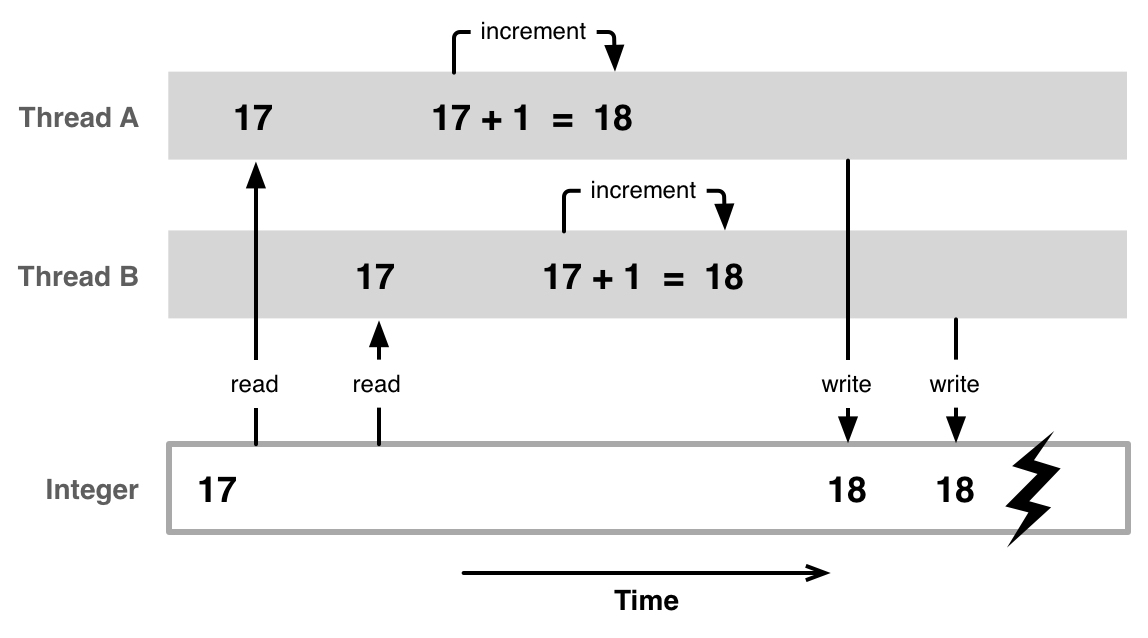
\includegraphics[width=\linewidth]{Images/race-condition.png}
                \caption{Basic Race Condition Example}
                \label{fig:race-condition}
            \end{figure}

            Languages not enforcing mutability/immutability in a manner that enforces best practice 
            of concurrency are potential breeding grounds for these vectors for attack as we move 
            rapidly to more and more concurrent computation in most devices as described and 
            suggested by Herb Sutter\cite{Herb-Sutter} in 2005.
            \medskip
            \\
            Rust\cite{Rust} and Golang\cite{Golang} prove to be exciting examples of the potential
            of concurrency, while both consuming more memory on systems, they offer languages 
            that enforce best practice with concurrency\cite{sima2012secure}, and in the case of Rust, immutability and
            the concept of ownership/borrows of variables/objects which leads to enforcing the 
            inability to modify the original value, or create copies of the value that do not
            reflect onto the original value.
            \medskip
            \\            
            Golang implements checking for potential deadlocks, channels which can be locked to send or receive only and job queuing by the use of wait groups for goroutines
            (effectively a concurrent call to a method that can be awaited or not) leading to 
            an ability to load a large number of tasks into a queue for processing and knowing 
            that using goroutines with pointers to a wait group that will ensure threads spawned
            from a goroutine are not deadlocked and have garbage collection performed on exit 
            using a defer method.
            \medskip
            \\
            Even for systems deemed legacy and only being supported in an extended lifetime setting, 
            frameworks for debugging and detection of race conditions have existed since the 
            late eighties\cite{savage1997eraser}\cite{balasundaram1989compile}

        \subsection{Improper Error Handling}
            Handling of errors can commonly be implemented incorrectly, most languages now off the 
            ability to check in specified contexts if an error occurs and apply code specifically 
            for the case an error occurs, this is excellent for developers, however can prove to 
            expose too much information in some settings as suggested by Tsipenyuk, Chess and McGraw\cite{tsipenyuk2005seven}
            \medskip
            \\
            Take the example of a simple website, registration of a user or an attempted login is 
            greeted by an error page served by the instance of Microsoft IIS hosting the application:

            \begin{verbatim}
You have an error in your SQL syntax; 
check the manual that corresponds to your 
MySQL server version for the right 
syntax to use near Donoghue
            \end{verbatim}

            For most users, this is a frustrating error that shouldn't occur, however malicious 
            entities will pounce on this information, given we can easily determine the hosting
            enviroment for a website, it isn't a stretch to assume the username entered: O'Donoghue
            has caused an error, and quickly we can realise vectors potentially exploitable to gain
            a foothold in a system as covered in \hyperref[sec:injection]{\color{blue}injection} attacks.
            \medskip
            \\
            Simply, a defined custom page to refer users to in the case of errors is a great method
            to limit ability for an entity to probe further at a solution, as often, the stack trace
            is only a small part of default error pages, often including full pathing of the 
            offending source code on the host machine, the version of add-on/package affected and 
            the hosting system.

        \subsection{Insecure Configuration / Using Components with Known Vulnerabilities}
            Revealing information about packages, language version and other data points suggested above can lead 
            to detection of either insecure of out-of-date configurations 
            which reveal further attack vectors on a system. This isn't a suggestion on hiding 
            out-of-date packages or language versions but instead a recommendation to always keep
            up to date with the most recently released versions of both languages but also any 
            packages or imported third party libraries used as also recommended by Tsipenyuk, 
            Chess and McGraw\cite{tsipenyuk2005seven}
            \medskip
            \\
            One of the best examples of this problem in recently history is the Equifax breach in which an 
            outdated and known vulnerable framework: Apache Struts was used within the technology stack at
            Equifax\cite{Equifax-Breach}, leading to in excess of 140M users data breached with a large portion 
            of the data containing personally identifying information.
            \\
            The only remedy to this issue is to ensure all systems are updated where possible, and teaching good 
            update habits to users. Sysadmins do not have much of an excuse in today's technology ecosphere with 
            numerous vendor provided or open source options for rolling updates out to numerous computers at once.

        \subsection{Function Level Access Controls}
            Most languages support either authentication with a defined authentication authority or decorators 
            for methods to suggest how a function may be accessed, often for the ease of access in development 
            functions, properties or methods will be marked with static where the language supports such or 
            unnecessarily marked public. While typically not a flaw that will allow an entity to breach a system without 
            further vectors to attack, commonly the breach of a system will include a number of exploits chained 
            in succession to allow an entity to breach the system.
            \medskip
            \\
            \subsubsection{Example}
                In 2014 a user going by secgeek\cite{secgeek} was able to exploit a lack of access control in the 
                Twitter Ad system, realizing interception of a request to delete his own credit card number from 
                the system allowed for modification of the request and a new request with alternate credit 
                card details which were not owned by secgeek to be deleted.

        \newpage
        \onecolumn
        \subsection{ReDoS / Regex Denial Of Service}
            Given the requirement for string filtering is extremely common in all applications,
            ReDoS or Regex Denial Of Service\cite{ReDoS} vulnerabilities are a very real threat in application security.
            A number of common defenses can be used against ReDoS attacks, application of 
            which are extremely simple:
            \begin{enumerate}
                \item Atomic grouping in Regex
                \item Regex lifetime limits
                \item Sanitisation of input (Although this defeats the reasons to allow for
                Regex patterns to be used and is very easy to not implement correctly)
            \end{enumerate}

            \subsubsection{Atomic Grouping}
                Atomic grouping in Regex is a group that when Regex is no longer utilising 
                the group is thrown away, and any tokens, or record of the grouping are discarded.
            \subsubsection{Regex Lifetime Limits}
                Lifetime limits are extremely simple in design, a regex process is allowed only 
                a set amount of time in which it can perform its task. Failure to meet this 
                leading to the process being killed.
            \subsubsection{Sanitisation of input}
                This solution to Regex patterns does go very much against the reasoning of 
                using Regex in the first place, but has some valid uses cases:\\
                Consider a user sign-up form on a webpage, the user isn't searching, but 
                using anything but Regex in this setting would be pure nightmare fuel for 
                any developer. A quick search of what patterns to use would yield pages such as
                regular-expressions.info\cite{RegularExpressions.info} and you'd quickly realise
                the rabbit-hole for a suitable Regex statement could be:

                \begin{verbatim}
\b[A-Z0-9._%+-]+@[A-Z0-9.-]+\.[A-Z]{2,}\b
                \end{verbatim}

                But just as easily, it could be: 

                \begin{verbatim}
\A(?:[a-z0-9!#$%&'*+/=?^_`{|}~-]+(?:\.[a-z0-9!#$%&'*+/=?^_`{|}~-]+)*
 |  "(?:[\x01-\x08\x0b\x0c\x0e-\x1f\x21\x23-\x5b\x5d-\x7f]
      |  \\[\x01-\x09\x0b\x0c\x0e-\x7f])*")
@ (?:(?:[a-z0-9](?:[a-z0-9-]*[a-z0-9])?\.)+[a-z0-9](?:[a-z0-9-]*[a-z0-9])?
  |  \[(?:(?:25[0-5]|2[0-4][0-9]|[01]?[0-9][0-9]?)\.){3}
       (?:25[0-5]|2[0-4][0-9]|[01]?[0-9][0-9]?|[a-z0-9-]*[a-z0-9]:
          (?:[\x01-\x08\x0b\x0c\x0e-\x1f\x21-\x5a\x53-\x7f]
          |  \\[\x01-\x09\x0b\x0c\x0e-\x7f])+)
     \])\z
                \end{verbatim}
                As suggested by Goyvaerts\cite{RegularExpressions.info}:
                \begin{displayquote}
                    "So even when following official standards, there are still trade-offs to be made. Don't blindly copy regular expressions from online libraries or discussion forums. Always test them on your own data and with your own applications."
                \end{displayquote}

                As shown by a \hyperref[sec:PyReDoS]{\color{blue}simple python script} the checking of 
                group bounds alone costs almost twice the time to be executed and realistically 
                does not give the application any more weight in being more accurate.
                \begin{table}[H]
                    \centering
                    \begin{tabular}{|l|l|}
                    \hline
                                              & Time(s)                \\ \hline
                    Simple Match (No Attack)  & 0.000187635421752  \\ \hline
                    Complex Match (No Attack) & 3.337860107421875  \\ \hline
                    Simple Match (Attack)     & 0.000261545181274 \\ \hline
                    Complex Match (Attack)    & 3.099441528320312 \\ \hline
                    \end{tabular}
                    \end{table}

                While these values don't seem extremely costly, they can quickly become extremely heavy in
                terms of computation required.

    \newpage
    \twocolumn
    \section{Modern Language Issues}
        \subsection{Issues Common in Python}
            Python recently proved to be one of the fastest growing languages based on responses to 
            the stackoverflow developer survey\cite{Stackoverflow-Survey} and while python is close to 
            twenty years old, it is considered a new language compared to the likes of C or Perl.

            As suggested by Wheeler\cite{Wheeler} a number of issues are inherent using python:
            \subsubsection{Lack Of Compile Time Checking}
                Issues related to the lack of compile time checking in python are a serious security
                concern as standard static analysis tools for auditing code for security issues 
                have a much more difficult time determining the suitability of code.
                \\
                It must be noted however, that unit tests and dynamic analysis / fuzzing can prove
                to be an excellent method to check python code for issues.

        \subsection{Issues Common in PHP}
            PHP is not my area of expertise, however a large number of recent exploits using 
            flaws in PHP have become a trend with the uptake of content generators such as WordPress.
            \subsubsection{Injection: register\_globals = ON}
                Register globals is a common resolution to many issues in developing PHP, however
                commonly it is left enabled in development or due to inexperience assumed to be okay to 
                leave set on the issue lies in any quest that depends on one of these globals set, say we are 
                checking if a user is an admin or not before allowing access to a section/page:

                \lstset{style=php}
                \begin{lstlisting}
                    if($admin) 
                    { 
                    // let them in 
                    } 
                    else 
                    { 
                    // kick them out 
                    }
                \end{lstlisting}\cite{Devshed-PHP}

                Issues arise when a user can inject this global into the request via:

                \begin{lstlisting}
                    script.php?admin=1
                \end{lstlisting}

                As suggested again by Wheeler\cite{Wheeler}, using version 4.2.0 of PHP or greater has 
                features enabled that mitigate most of the danger around this issue.

    \section{Mature Language Issues}
        \subsection{C/C++}
            \subsubsection{Overflow/Underflow Issues}
                C and C++ are notorious for the issue of overflows, overflows can easily 
                cause potential vectors for malicious entities to perform a number of 
                attacks.
                The most common attacks on overflow issues include arbitrary code execution,
                a basic example thanks to lapk\cite{lapk}:

                \lstset{style=cplusplus}
                \begin{lstlisting}
                    #include <iostream>
                    int main( void )
                    {
                    int authentication = 0;
                    char cUsername[ 10 ];
                    char cPassword[ 10 ];

                    std::cout << "Username: ";
                    std::cin >> cUsername;

                    std::cout << "Pass: ";
                    std::cin >> cPassword;

                    if( std::strcmp( cUsername, "admin" ) == 0 && std::strcmp( cPassword, "adminpass" ) == 0 )
                    {
                    authentication = 1;
                    }
                    if( authentication )
                    {
                    std::cout << "Access granted\n";
                    std::cout << ( char )authentication;
                    }
                    else
                    {
                    std::cout << "Wrong username and password\n";
                    }

                    return ( 0 );
                    }
                \end{lstlisting}

                Where in this example, no checking of input bounds is performed when the user has 
                entered data that exceeds the size allocated to username (Char[10]) so as suggested 
                in lapk's\cite{lapk} example, the input of "0123456789abcdef1" would easily overflow
                the bounds of the referenced memory. In the case of a compiled x64 binary compiled for 
                Windows the above code would set authentication to 1 despite the comparisons made between password and the expected value.
                \\
                What is curious about the above example, is it also exhibits two other blatant 
                development flaws\cite{OWASP-SCP-Quick-Reference-Guide-v2}: 
                \begin{itemize}
                    \item Secrets within source code - easily avoided when stored in a DB or loaded
                    from a file outside of source control
                    \item Failure to set authentication = 0 / false when the failure of comparison 
                    occurred.
                \end{itemize}
                While it must be noted that the example is more for educational purposes than how an 
                application should be written.

                Overflows and underflows are covered well by the OWASP Secure Coding Practices
                Reference Guide\cite{OWASP-SCP-Quick-Reference-Guide-v2} and further suggestions 
                for defenses and good practice include: 
                \begin{itemize}
                    \item Truncation of input to fit destination (exceptions may occur here however and values such as passwords should always include as large as possible an allocation rather than truncating data)
                    \item Avoidance of functions that are considered unsafe, printf, strcat and 
                    strcpy are all good examples of this in C/C++
                    \item Ensure all memory that is no longer considered in-scope is cleared, this 
                    is easier said than done and languages such as Golang\cite{Golang} implement 
                    excellent methods in which to ensure this function is performed (Defer in Golang)\cite{Golang-Defer}
                \end{itemize}

    \newpage

    \printbibliography

    \newpage
    \onecolumn

    \appendix
    \section{Appendix}
        \subsection{Proof Of Concept Code}
            \subsubsection{Python ReDoS}
            \label{sec:PyReDoS}
            \_
            \medskip
                \pythonexternal{Resources/regex.py}

    \end{document}
